\chapter{Related Work}
\label{chapterlabel2}

\section{CTR Prediction}
Click-Through Rate (CTR) prediction is a well-studied online advertising problem in recent years. Advertisers tend to use CTR as a metric for the evaluation of the performance effectiveness of online advertising system to better predict their cost and revenue economically. CTR prediction is important for both sponsored search and RTB industry. 
Billions of dollars are being spent on sponsored advertising a year, predicting the possibility of the click for a specific ad in response to a certain query from the user is crucial to the business model of search engine industry. For sponsored search, in \cite{richardson2007predicting}, Microsoft tends to build a ML model making use of the features of ads, terms, and advertisers to predict the click probability for new ad, which can not only increase the revenue of the website, but also the user satisfactory. Logistic regression model is used to train the historical information of the ads and it is used to predict the CTR of new ad. It also shows that the position of the ad on the webpage largely decides the attraction of the ad. \cite{graepel2010web} shows an \textit{adPredictor} model to interpret the CTR as a linear combination of weighted features to realize a Bayesian online algorithm, the weights space is regarded as a Gaussian prior distribution and its mean and variance can be updated with the income of new data. \cite{zhu2010novel} proposes a General Click Model (GCM) upon a Bayesian network and \textit{Expectation Propagation} method is used to perform approximate Bayesian inference. It shows that all the other models are just the special cases of GCM. \cite{mcmahan2013ad} proposes a system which aims to train massive models on massive data with minimum resources, the linear model of logistic regression is used, but a new way of regularization which is similar to Regularized Stochastic Learning (RDA) is realized for gradient descent. This method is easier to implement and able to improve the final accuracy. As a trick, the method of probabilistic feature inclusion is used to select the features which can be used to avoid the long-tailed distribution of features, thus improving the accuracy of prediction and save the memory of machines meanwhile.

Besides sponsored search, many companies also set foot in RTB industry, Google provides a detailed and comprehensive report about the industry\cite{google2015}, since we are standing at the age of the intersection of data liquidity and inventory liquidity with the rise of exchangers and advertisers who have brought much more liquidity for the market, advertisements have a huge amount of ways to be presented to the potential audience, RTB is a revolutionary business model for display advertisement, as shown in Figure \ref{fig:ctr} the media buyers do not need to buy the advertising slots from millions of individual sites which is operationally impossible, but from a single DSP. A more efficient, faster and automated way is realized by RTB for advertisers to buy slots among sites more easily. 

Many researches in the field of RTB have been done. Besides the common linear model , non-linear model, such as tree based models and deep learning are all used for the CTR prediction in the context of RTB. In \cite{agarwal2010estimating} LMMH (Log-linear Model for Multiple Hierarchies) is proposed to solve the problem of estimating CTR for high dimensional and multivariate categorical data, the tree-like model is used in which the weight for each pair of node can be stored so that the click probability can be modelled as a product of the weights for all the pairs of nodes. \cite{trofimov2012using} proposes a boosting tree method which is a MatrixNet machine learning algorithm showing better performance than linear and logistic regression model. \cite{he2014practical} combines decision tree and logistic regression model together, the fundamental idea is to transform the original feature space into the \textit{right} feature space using boosting tree model, the right feature space can highly improve the CTR prediction performance in terms of AUC, instead of manually processing of feature selection and combination, boosting tree is able to generate the appropriate features which are the leafs of the tree. In order to keep the freshness of model, the model will be trained on a daily basis. It shows that the the combination of decision tree and logistic regression model can generate the right features, as well as using the right model, which will perform much better than selecting high value features and complex model.

\begin{figure}[h]
\centering
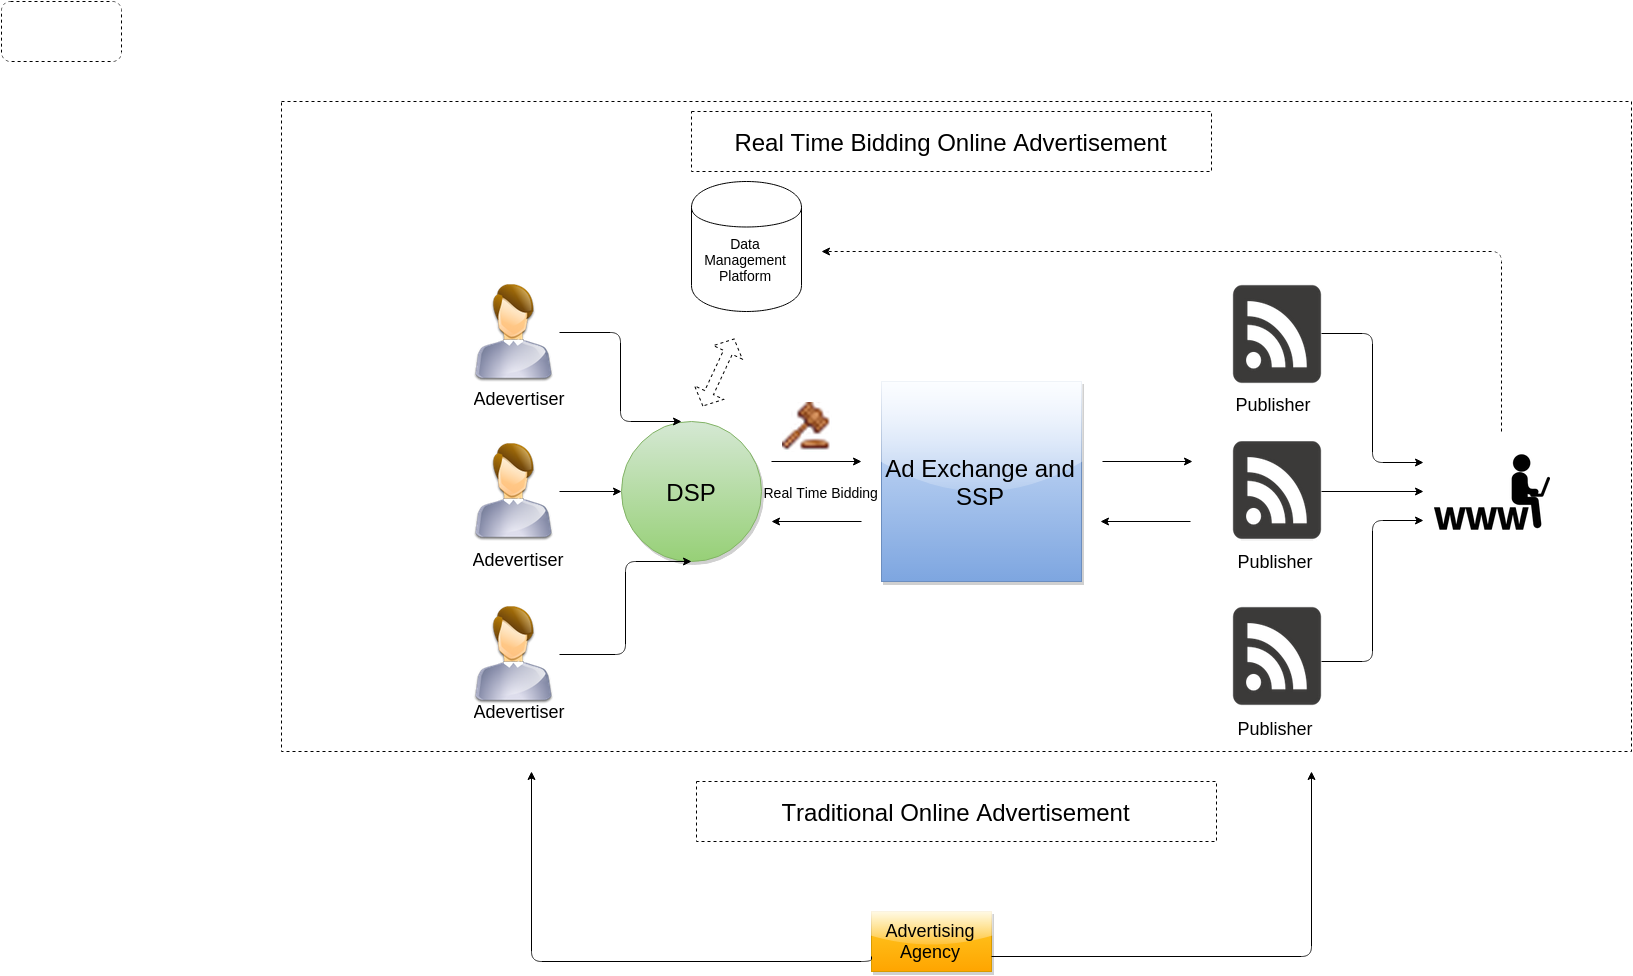
\includegraphics[width=\columnwidth]{rtblanscape.png}
\caption{Comparison between Real Time Bidding and Traditional Online Advertising}
\label{fig:ctr}
\end{figure}

\cite{cheng2012multimedia} conducts an experiment on over billions of impressions. There are also other researches on CTR prediction problem, \cite{richardson2007predicting} makes use of logistic regression to predict clicks. \cite{mcmahan2013ad} discusses on the practical engineering of CTR estimation as well as the performance of applying traditional machine learning model on complex huge dataset. \cite{zhu2010novel} discusses on General Click Model based on Bayesian network. \cite{graepel2010web} talks about \textit{Online Bayesian Probit Regression}. \cite{mohan2011web} discusses on the use of \textit{Gradient Boosting Regression Tree} (GBRT) on web ranking. GBRT algorithm is commonly used in the industry now, which is a non-linear classifier composed of a set of separators, by stacking a GBRT with LR to eliminate the non-linearity in the features it is able to give better CTR prediction results.

In conclusion, the researches on CTR are abundant for linear or non-linear regression model for sponsored search and RTB, namely how to find the \textit{right model}. However, in real industry, due to the unstructured and complex characteristic of the data, the pre-processing of data before putting into the model is more important for a real-world CTR prediction, the researches on \textit{Feature Engineering} is rare, and most of them is in the field of \textit{Natural Language Processing} (NLP), such as in \cite{garla2012ontology}, which makes use of the domain knowledge in biomedical to encode in the \textit{Unified Medical Language System} so that the machine learning clinical text classification performance can be improved largely. As said by Mohammad Pezeshki in \cite{featureengineering}

\textit{Actually the success of all Machine Learning algorithms depends on how you present the data.}

A good feature engineering means, the feature space is more flexible and easier, which means less complex model can be used but still obtain good performance, as the work in \cite{he2014practical}, the binary feature space is transformed into a lower dimension space using decision tree. Similar, in our paper, contrary to most of the researches in CTR prediction problem which focus on ML models, we will turn our focus on a more fundamental problem, namely how to prepare a better feature space for the model training.   

\section{Cold Start Problem}
The main purpose of this paper is to solve the cold start problem for CTR prediction, namely we use the data from old advertisement campaigns to predict the CTR in the new advertisement campaigns. Considering the complex and unpredictable of human behavior, this is a complicated problem. Few researches have been done to solve the cold start problem in the field of online advertising, therefore we will start to research on cold start problem in the area of \textit{recommendation system} with more abundant resources.

Cold start is a classical problem in the field of recommendation system, it focuses on the issues when the system is at the start stage without enough information so no inferences for users or items can be drew. \textit{Collaborative Filtering} (CF) is the most popular method proposed to solve this problem. In \cite{schein2002methods}, content and collaborative data are combined to solve the problem under a single probabilistic framework. \cite{su2009survey} provides a comprehensive review of collaborating filtering methods, model-based, memory-based and hybrid CF algorithms are discussed in this paper. There are also some papers focusing on solving the cold start problem based on the data itself. \cite{li2013news} proposes a personalized news recommendation model to apply ranking on hypergraph that includes users, news articles, and topics. The motivation that the researcher apply the hypergraph in news personalized recommendation is that for a news recommendation system, mining implicit relations among users, news articles, topics and named reading community is important. Given the special properties of the news articles, the researchers partition the hypergraph into multiple fine-grained 
ones, and then transform the recommendation problem into a ranking problem among the fine-grained hypergraphs. After that, the similarity graph of the news articles are built, namely setting the weights of the hyperedge. Finally, the transductive inference is performed on the news capsule in order to derive the news based on the user’s preference to provide the recommendation list for the user. \cite{jiang2012social} addresses the problem of sparsity and cold start in social recommendation. The researchers propose a \textit{Hybrid Random Walk} (HRW) algorithm to integrate multiple heterogeneous domains using signed/unsigned links,directed/undirected links and within-domain/cross-domain links into a star-structured hybrid graph in which user graph is at the center. A random walk is performed until its convergence and the steady state distribution is used for recommendation. \cite{feng2012incorporating} proposes a supervised random walk for setting of personalized tag recommendation. In this article, the heterogeneous information in the social tagging system, such as users’ tagging behaviors, tag semantics, social networks and item profiles are implemented to help alleviate the cold start problem due to data sparsity.

The above researches all focus on recommending novel items to the users based on information from heterogeneous information sources, they are not directly related to CTR prediction directly since the authors all regard data as vertex and use edge to represent the relations between the data, but we can get the insights from the literature that the information from old domains can be somewhat transformed to the new domain for the recommendation of new item. Since we can regard CTR prediction problem as a typical recommendation problem, in which advertisements with higher probability to be clicked will be recommended to the users. Therefore based on the information from the user, the advertisement itself, and the context information, we can find the position of the user profile in the network organized by these information, which confirms the certain level of generalization of the data distribution among all the domains. Therefore, it is possible to predict the CTR for new users based on the historical data as long as the logical relations exist between the historical data and the new user. 

The only paper focusing on cold start problem in the field of online advertising is \cite{agarwal2009regression}, which proposes a \textit{Regression Latent Factor} to incorporate entity features into latent factor learning. In this way the historical data and new item data can be combined together to improve the generalization of the model. We can conclude that getting the comprehensive information from history and to some point make use the new information will be a feasible way to solve the cold start problem for CTR prediction.

\section{Domain Adaptation}
In order to solve the cold start problem, we need to make use the old information in history. In the aspect of online advertising, it means how to transform the knowledge from source domains, namely old campaigns to the target domain, which is the new campaign.

The concept of domain adaptation is derived from \textit{Transfer Learning}, transfer learning is a popular research topic in the fields of artificial intelligence, machine learning, NLP, etc. In the field of machine learning, different from traditional predictive machine learning methods which ignore the difference between training and test datasets, in real world, the source and target sets should suffer from the situation of \textit{dataset shift} \cite{quionero2009dataset}, therefore, transfer learning will play a role to transfer the knowledge from current advertisement campaigns to the new ones. 

\cite{pan2010survey} makes a detailed discussion on transfer learning focusing on categorizing transfer learning for regression, classification and clustering problems. When the source and target tasks are different, and the source and target domains are same, it is called \textit{inductive transfer learning}, when the source and target domains are different however the source and target tasks are the same, it is called \textit{transductive transfer learning}. The final goal of the transfer learning system is to equip the system with the ability to recognize and apply the knowledge learned in previous domains to novel ones, which share some point of commonality. \cite{dai2007transferring} proposes a method to solve the problem of transfer learning in text classification using an EM-based naive Bayes classifier, the initial probability distribution of the source domain is estimated and then the EM algorithm is used to revise the trained model for the test dataset distribution using the unlabeled instances, this research with \cite{jiang2007instance}, \cite{huang2006correcting} and \cite{bickel2007discriminative} can be regarded as the \textit{instance based approach}. The assumption of this approach is that the source and target domains own many overlapping features, the items in the source domain will be regarded as the samples from the target domain, and part of the labeled data in the source domain can be reused in the target domain after re-weighting, the a rejection process will be made and the samples will be re-weighted again to map the target domain to the source domain to make the distributions similar. In this way, an adaptive feature representation should be developed to overcome the difference between the source and target domains. 

Another approach is \textit{feature representation transfer}, such as the researches in \cite{dai2007co}, \cite{ando2005high}, and \cite{blitzer2006domain}. In \cite{dai2007co}, a co-clustering algorithm is proposed to classify out-of-domain documents, the class label information given by the source domain can be extracted to label the word clusters for target domain. In \cite{blitzer2006domain} the domain adaptation problem in sentiment classification is discussed. No labeled data for the new domain is needed, at first \textit{N} pivot features are identified, then \textit{N} classifiers are built to predict the pivot features from remaining features, after that by computing the top eigenvectors the shared feature space can be discovered, and then the classifiers can be trained on the source domain using the augmented features. In brief, the approach of \textit{feature representation transfer} is based on the assumption that the source and target domains only share a part of the features, so the difference between the two domains can be solved by minimising the distances between the two domains, or using a multitask model to optimize the feature spaces of the two domains. In \cite{pan2011domain} the authors map the source and target domain data to the latent space spanned by the factors which can reduce domain difference and preserve original data structure. \cite{gao2008knowledge} is an example of the method \textit{parameter transfer}, which aims to discover the shared parameters or priors between the source and target domains. This approach is based on the assumption that the marginal distribution of feature space for target-domain and source-domain are similar, and also conditional probabilities also ought to be similar. In this way the parameter learned from the source domain can benefit the model for target domain. 

Our focus of this paper is to make use of transfer learning for CTR prediction problem of new advertisement campaigns. For the CTR problem, it is reasonable to say tasks between old and new campaigns are the same, which is a binary prediction classifier, however, the domains of the two will be distinct due to different data distribution and feature sets. 

From the above literature, we can make the following conclusions that we can refer to for our research. Firstly, the feature spaces of the source and target domains should be somewhat related, only if then can we transfer the knowledge learned from the source domain to the target domain, this is reasonable for the CTR problem, since even though the feature distribution from the old advertisement campaign and the new campaign can be different, the human behaviors should be related, namely the advertisements which can induce people to click should have some commonality. Secondly, the knowledge of the feature space and parameters from the model from the source domain can both benefit the CTR prediction model training in target domain. 

We also borrow the concept of \textit{domain shift} during our experiment, the comprehensive introduction of domain shift can be shown in the book \cite{quionero2009dataset}. The domain shift happens when the distribution of dataset changes arbitrarily, so the training data cannot be used directly to make predictions on the test domain. In this paper we will focus on \textit{covariate shift}, with the situation that \(Pr_{source}(x,y)\) and \(Pr_{target}(x,y)\) only differ in the marginal distribution of covariate \cite{zhang2013domain}, in the paper, we propose a machine learning method to quickly check whether the covariate shift exists between source and target datasets, ignited by the idea from \cite{coviriate}.






 










